Este capítulo presenta los resultados disponibles y los interpreta en relación con los objetivos. Las afirmaciones se limitan a la configuración evaluada.

\section{Caracterización del conjunto de datos}

El conjunto consolidado contiene 20.025 registros a nivel bloque-mes y veintiún características numéricas. La distribución reportada para la variable objetivo es de 17.010 registros sin crisis (85\%) y 3.015 con crisis (15\%). Esta proporción evidencia un desbalance que hace necesario interpretar la exactitud junto con precision, recall y AUC-ROC.

\begin{table}[H]
    \centering
    \begin{tabular}{|l|r|r|}
    \hline
        \textbf{Clase} & \textbf{Registros} & \textbf{Proporción} \\
    \hline
        No crisis & 17.010 & 85\% \\
    \hline
        Crisis & 3.015 & 15\% \\
    \hline
        \textbf{Total} & 20.025 & 100\% \\
    \hline
    \end{tabular}
    \caption{Distribución global de la variable objetivo.}
    \label{tab:dist_objetivo}
    \end{table}

El número de registros agregados no equivale directamente al número de secuencias utilizadas para entrenar los modelos. La versión original menciona 293 muestras de entrenamiento, pero no incluye los conteos necesarios para reproducir la transformación. Por esta razón, la muestra efectiva y la distribución por horizonte deben verificarse antes de considerar definitiva la evaluación.

\section{Resultados del procesamiento y \newline análisis exploratorio}

\subsection{Correlaciones}

La Figura 5.1 muestra correlaciones elevadas entre algunas variables. En particular, el documento original reporta una relación cercana a 1 entre \texttt{num\_creditos} y \texttt{creditos\_cerrados}, así como entre \texttt{monto\_total} y \texttt{monto\_promedio}. Estas relaciones pueden generar redundancia, aunque la multicolinealidad no afecta de la misma manera a árboles y redes neuronales. Los valores de VIF (del ingles Variance Inflation Factor) mencionados en la versión original no se conservan como evidencia principal porque no se documenta su cálculo completo.

\begin{figure}[H]
    \centering
    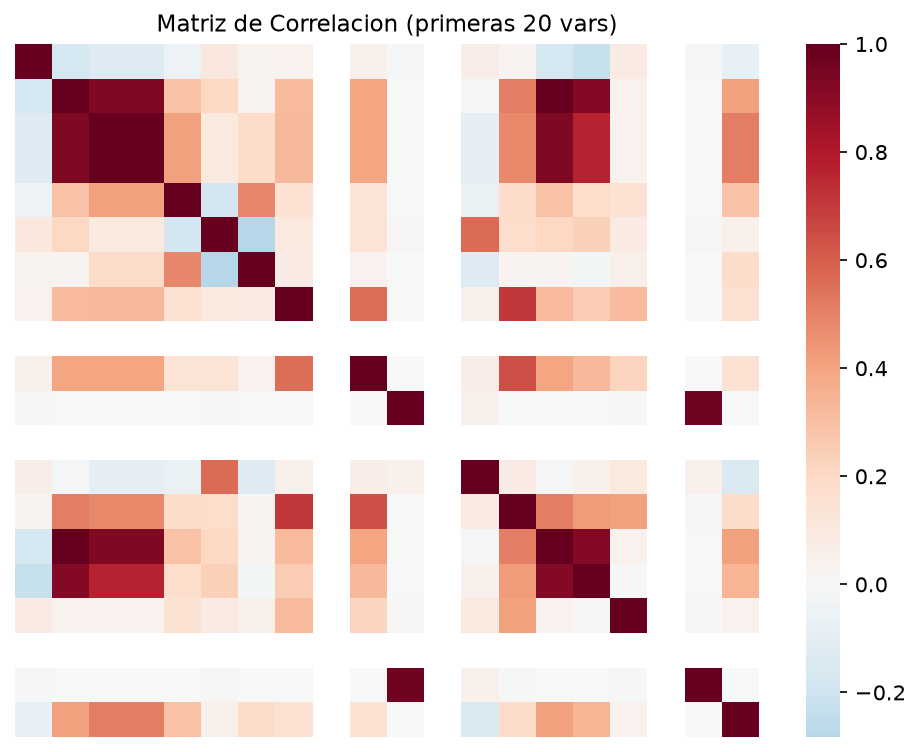
\includegraphics[width=0.8\textwidth]{images/01_heatmap_correlaciones.png}
    \caption{Matriz de correlaciones de Pearson entre las 21 características numéricas del conjunto analítico. Los valores cercanos a 1,0 (color intenso) indican alta correlación positiva. Se observa multicolinealidad severa entre pares como \texttt{num\_creditos}--\texttt{creditos\_cerrados} y \texttt{monto\_total}--\texttt{monto\_promedio}. La multicolinealidad afecta de manera diferente a modelos lineales y no lineales.}
    \label{fig:heatmap}
\end{figure}

\subsection{Poder predictivo individual}

El análisis univariado identifica \texttt{tasa\_judicial} y \texttt{creditos\_judiciales} como las variables con mayor AUC-ROC individual. Las categorías cualitativas ``muy alto'' y ``medio'' se eliminan porque la tesis no define umbrales formales para ellas.

\begin{table}[H]
    \centering
    \begin{tabular}{|l|r|}
    \hline
    \textbf{Variable} & \textbf{AUC-ROC individual} \\
    \hline
        tasa\_judicial & 0,926 \\
    \hline
        creditos\_judiciales & 0,912 \\
    \hline
        saldo\_promedio & 0,666 \\
    \hline
        monto\_total & 0,651 \\
    \hline
    \end{tabular}
    \caption{Variables con mayor AUC-ROC individual según el análisis exploratorio.}
    \label{tab:auc_individual}
    \end{table}

\begin{figure}[H]
    \centering
    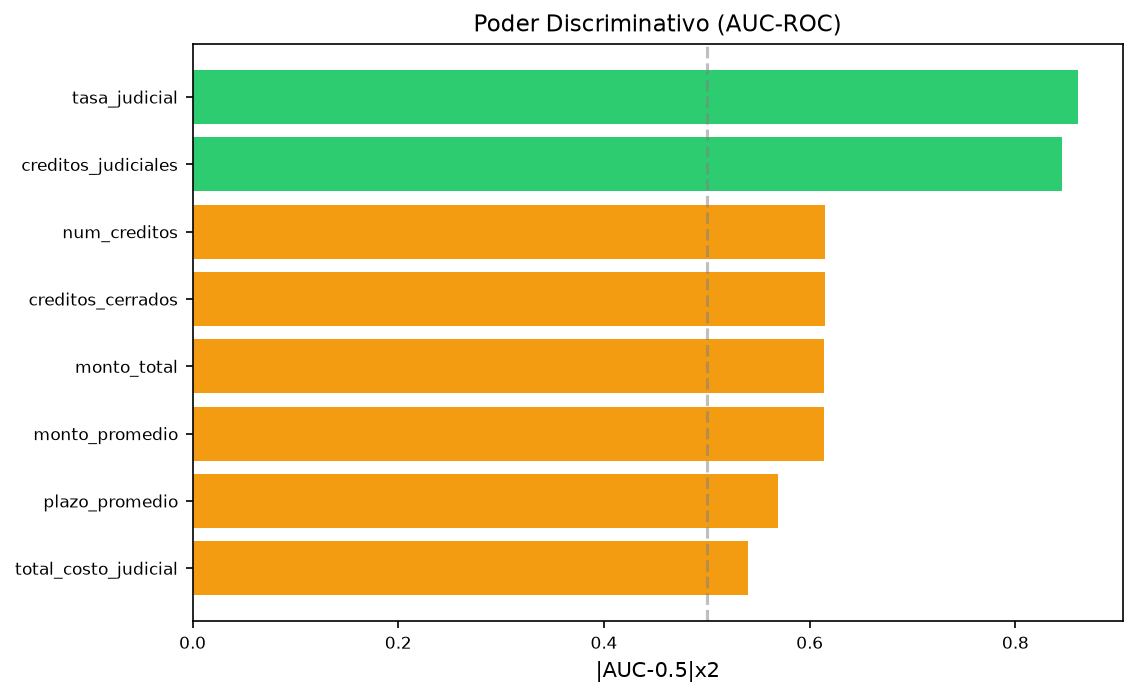
\includegraphics[width=0.8\textwidth]{images/09_auc_roc_variable.png}
    \caption{AUC-ROC calculada individualmente para cada variablepredictora, evaluada contra la etiqueta \texttt{crisis\_flag}. El AUC-ROC mide la capacidad de cada variable para distinguir entre bloques con y sin crisis, sin considerar interacciones con otras variables.}
    \label{fig:auc_roc}
\end{figure}

Estos resultados requieren una lectura prudente. Una alta capacidad discriminativa de variables judiciales puede ser válida si la información está disponible antes del horizonte predicho; también puede revelar fuga de información si esas variables forman parte de la etiqueta o reflejan un evento contemporáneo. Sin las ocho reglas de \texttt{crisis\_flag}, no es posible distinguir entre ambas explicaciones.

\subsection{Evolución temporal de la clase positiva}

La Figura 5.3 muestra cambios en la proporción de crisis a lo largo del periodo. El documento original describe niveles de 5--7\% antes de 2020, un pico de 20--24\% durante 2020--2021 y una estabilización cercana al 15\% posteriormente. Esta coincidencia temporal no permite atribuir el cambio a la pandemia sin un análisis causal y fuentes externas; por ello, se reporta únicamente como patrón descriptivo.

\begin{figure}[H]
    \centering
    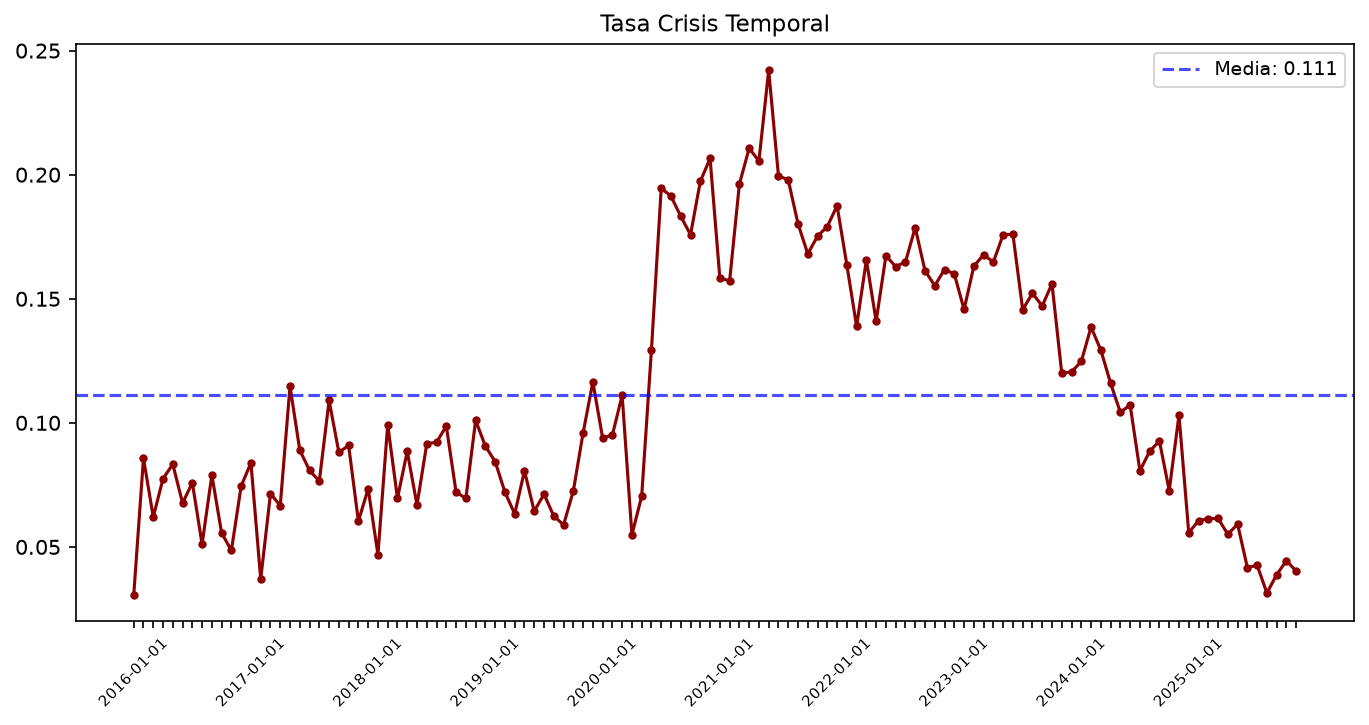
\includegraphics[width=0.8\textwidth]{images/07_tasa_crisis_temporal.png}
    \caption{Evolución mensual de la proporción de bloques etiquetados como crisis (\texttt{crisis\_flag}=1) en el periodo 2015--2026. Se observa un incremento en el periodo 2020--2021 seguido de una estabilización. Esta descripción es únicamente observacional; no se establece relación causal con eventos externos.}
    \label{fig:crisis_temporal}
\end{figure}

\section{Resultados de los modelos}

\subsection{LightGBM}

LightGBM produjo resultados para los dieciocho horizontes. La Tabla 5.3 reproduce los horizontes documentados y el promedio reportado. El AUC-ROC disminuye de 0,874 a un mes a 0,702 a dieciocho meses. El recall se reduce de 0,542 a 0,034, lo que indica que, con el umbral utilizado, el modelo identifica muy pocos casos positivos en el horizonte más largo.

\begin{table}[H]
    \centering
    \small
    \begin{tabular}{|l|r|r|r|r|}
    \hline
    \textbf{Horizonte} & \textbf{Accuracy} & \textbf{Precision} & \textbf{Recall} & \textbf{AUC-ROC} \\
    \hline
        1 mes & 0,937 & 0,694 & 0,542 & 0,874 \\
    \hline
        3 meses & 0,942 & 0,837 & 0,512 & 0,869 \\
    \hline
        6 meses & 0,927 & 0,632 & 0,525 & 0,838 \\
    \hline
        12 meses & 0,906 & 0,447 & 0,369 & 0,765 \\
    \hline
        18 meses & 0,897 & 0,500 & 0,034 & 0,702 \\
    \hline
        \textbf{Promedio} & \textbf{0,917} & \textbf{0,571} & \textbf{0,391} & \textbf{0,800} \\
    \hline
    \end{tabular}
    \caption{Métricas reportadas para LightGBM en horizontes seleccionados.}
    \label{tab:lgbm_metricas}
    \end{table}

\begin{figure}[H]
    \centering
    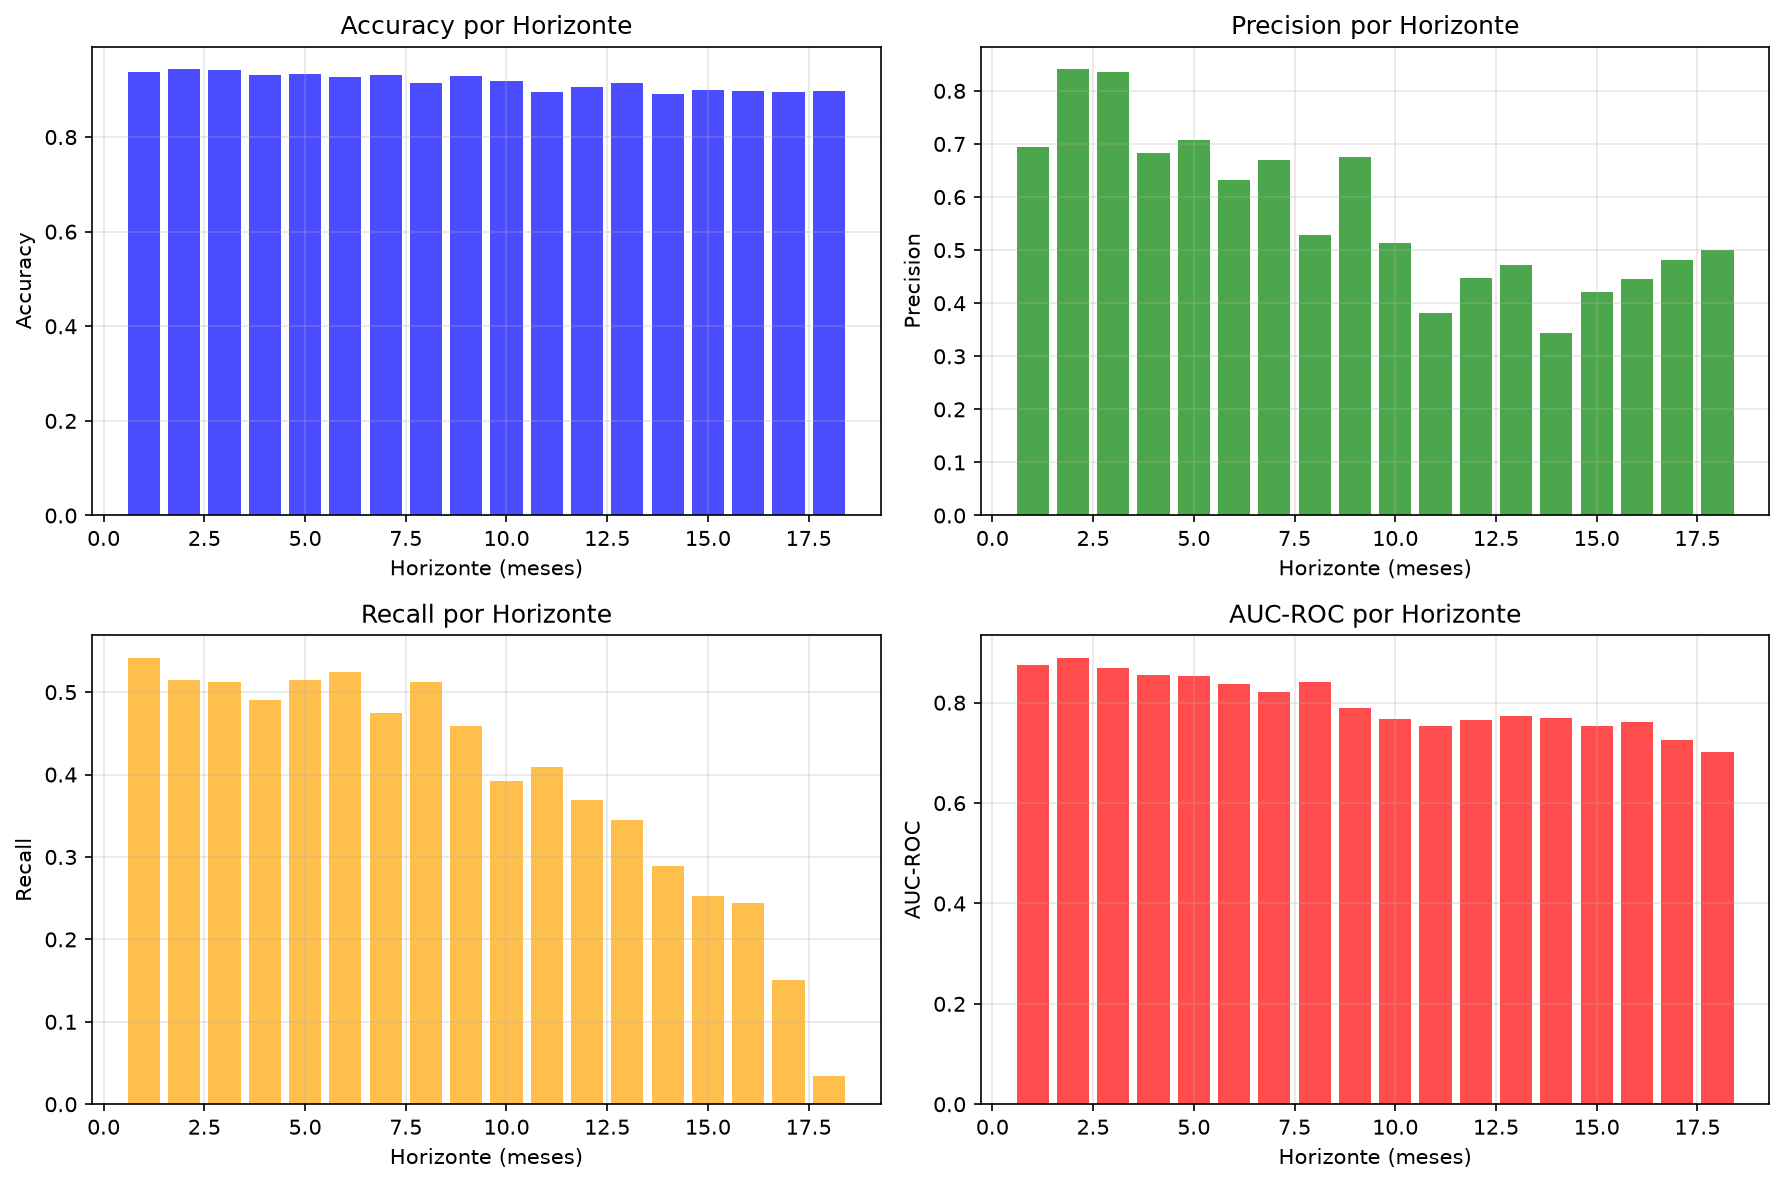
\includegraphics[width=1.0\textwidth]{images/lgbm_metricas_por_horizonte.png}
    \caption{Evolución de las métricas de LightGBM a través de los horizontes evaluados.}
    \label{fig:lgbm_metricas}
\end{figure}

La Figura 5.5 muestra la importancia interna de las características. La predominancia de variables judiciales coincide con el análisis univariado, pero no demuestra causalidad ni garantiza que la señal esté disponible antes de la predicción.

\begin{figure}[H]
    \centering
    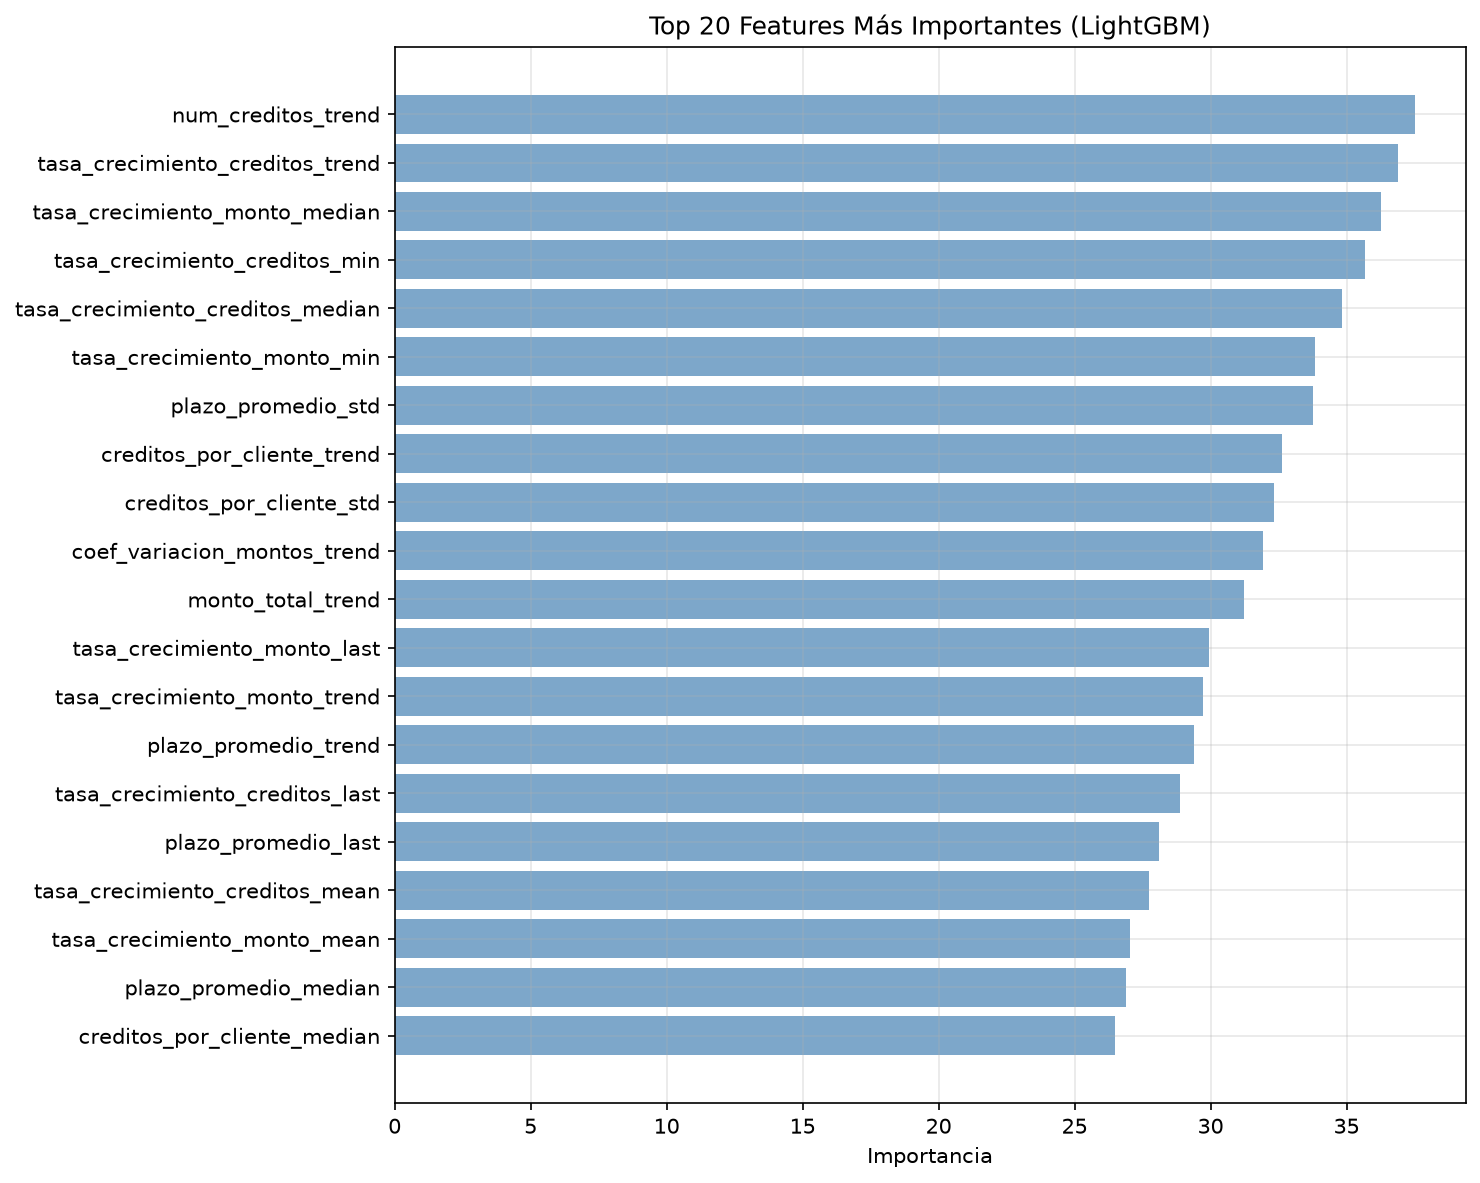
\includegraphics[width=1.0\textwidth]{images/lgbm_importancia_features.png}
    \caption{Importancia de características reportada por LightGBM (``split importance''). El método cuenta la cantidad de veces que cada variable se utiliza para dividir nodos en todos los árboles del ensemble. Las variables judiciales (\texttt{tasa\_judicial}, \texttt{creditos\_judiciales}) predominan, lo cual puede reflejar tanto poder predictivo real como dependencia con la etiqueta \texttt{crisis\_flag} (ver Sección 4.5).}
    \label{fig:lgbm_features}
\end{figure}

\subsection{CNN}

La implementación de CNN reportó un AUC-ROC de 0,50 y una pérdida que se mantuvo alrededor de 12,5. También se observaron oscilaciones extremas en accuracy, precision y recall, compatibles con predicciones concentradas en una sola clase. Un AUC-ROC de 0,50 indica ausencia de discriminación en la evaluación; por sí solo no demuestra una causa ni permite concluir que todas las CNN sean inadecuadas para este problema.

\begin{figure}[H]
    \centering
    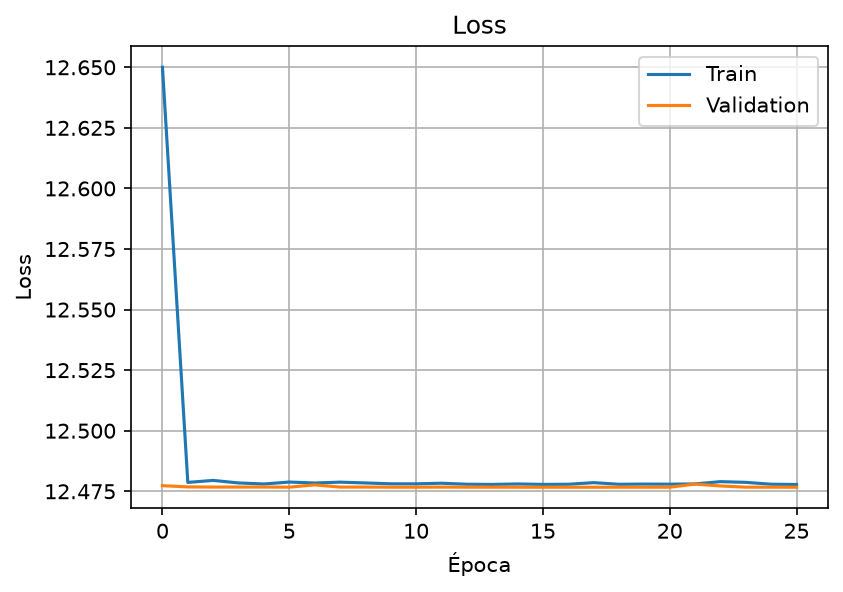
\includegraphics[width=0.8\textwidth]{images/cnn_loss.png}
    \caption{Curva de pérdida (\texttt{binary\_crossentropy}) durante el entrenamiento de la CNN. La línea continua representa la pérdida en entrenamiento y la discontinua la pérdida en validación (\texttt{val\_loss}). La pérdida se estabiliza en valores elevados ($\sim$12,5), lo que indica que el modelo no logra aprender una discriminación efectiva entre clases.}
    \label{fig:cnn_loss}
\end{figure}

La magnitud de la pérdida requiere revisar la función utilizada, las dimensiones de etiquetas y salidas, el escalado, los pesos de clase y el tamaño de lote. Estos elementos no están documentados con suficiente detalle para identificar el origen del comportamiento.

\subsection{MLP}

El MLP reportó una pérdida cercana a 12,47, AUC-ROC de 0,50 y predicciones concentradas en la clase no crisis, con precision y recall iguales a cero para la clase positiva. Este resultado describe el comportamiento de la implementación evaluada, pero no identifica sus causas. Entre los factores plausibles se encuentran el desbalance, el número de secuencias, la configuración de la pérdida, los pesos de muestra, el escalado y el ajuste de hiperparámetros.

\section{Comparación global}

La Tabla 5.4 corrige la inconsistencia de la tabla original: los valores de LightGBM son promedios de horizontes y no corresponden exclusivamente al horizonte de un mes. CNN y MLP se presentan con los valores globales reportados, por lo que la comparación no reemplaza una tabla completa por modelo y horizonte.

\begin{table}[H]
    \centering
    \begin{tabular}{|l|r|r|r|r|}
    \hline
    \textbf{Modelo} & \textbf{Accuracy} & \textbf{Precision} & \textbf{Recall} & \textbf{AUC-ROC} \\
    \hline
    LightGBM, promedio & 0,917 & 0,571 & 0,391 & 0,800 \\
    \hline
    CNN, resultado global & 0,090 & 0,090 & 1,000 & 0,500 \\
    \hline
    MLP, resultado global & 0,910 & 0,000 & 0,000 & 0,500 \\
    \hline
    \end{tabular}
    \caption{Comparación de los resultados reportados. Las unidades de resumen no son completamente equivalentes entre modelos.}
    \label{tab:comparacion}
    \end{table}

Bajo el criterio implementado de AUC-ROC promedio, LightGBM fue seleccionado para el flujo de inferencia. La selección es coherente con los resultados disponibles, pero debe considerarse provisional por cuatro razones: no se documentan repeticiones; no existe una prueba estadística; el ajuste de hiperparámetros no fue equivalente; y las salidas de LightGBM y de las redes se estructuran de manera diferente.

\section{Ejecución automatizada y registro}

El pipeline de Airflow produjo una ejecución posterior con accuracy promedio de 0,878 y AUC-ROC promedio de 0,846, mientras que el entrenamiento inicial reportó 0,917 y 0,800, respectivamente.

\begin{table}[H]
    \centering
    \begin{tabular}{|l|r|r|}
    \hline
    \textbf{Métrica} & \textbf{Ejecución inicial} & \textbf{Ejecución automatizada} \\
    \hline
        Accuracy promedio & 0,917 & 0,878 \\
    \hline
        AUC-ROC promedio & 0,800 & 0,846 \\
    \hline
    \end{tabular}
    \caption{Resultados reportados para las ejecuciones inicial y automatizada.}
    \label{tab:inicial_vs_final}
\end{table}

La diferencia no debe atribuirse a Apache Airflow. Airflow orquesta el procedimiento, pero no mejora por sí mismo un modelo. La variación puede relacionarse con cambios en datos, particiones, configuración o aleatoriedad; estos factores no quedaron documentados. El resultado sí evidencia que el flujo automatizado fue capaz de ejecutar el entrenamiento y registrar una salida.

\begin{figure}[H]
    \centering
    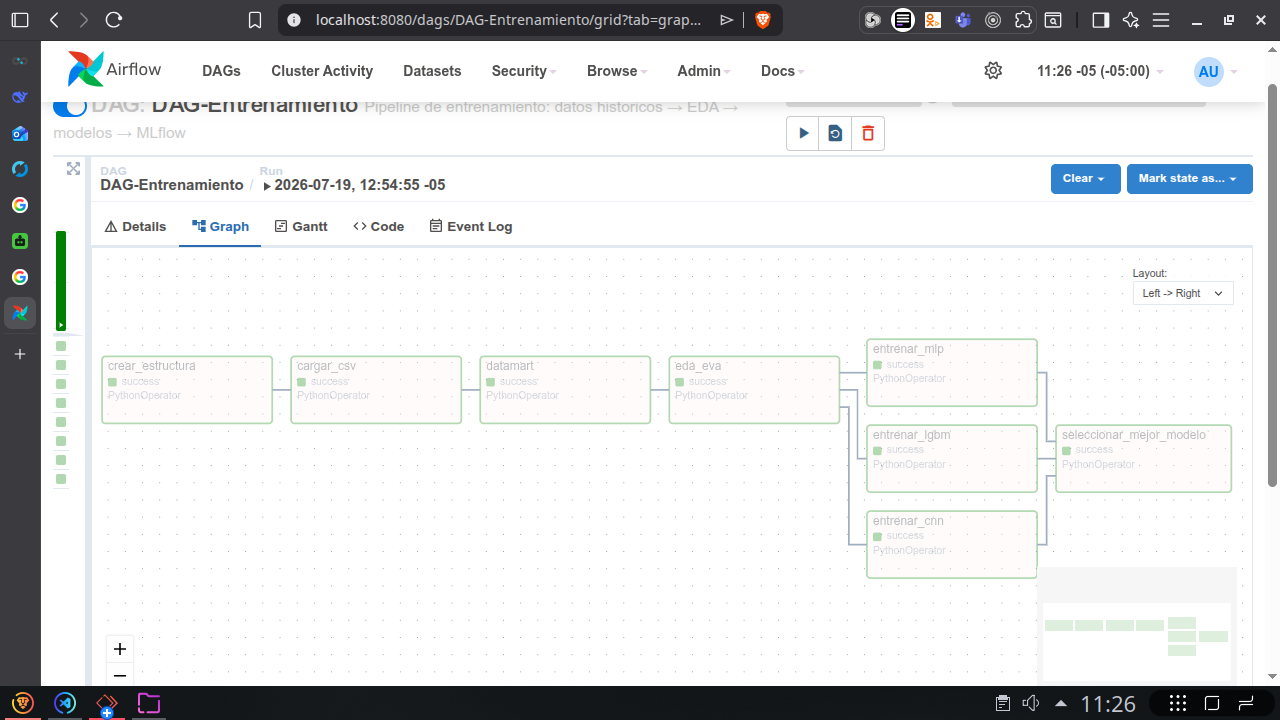
\includegraphics[width=0.8\textwidth]{images/dag-01entrenamiento.png}
    \caption{Vista del DAG de entrenamiento implementado en Apache Airflow.}
    \label{fig:dag_entrenamiento}
\end{figure}

\begin{figure}[H]
    \centering
    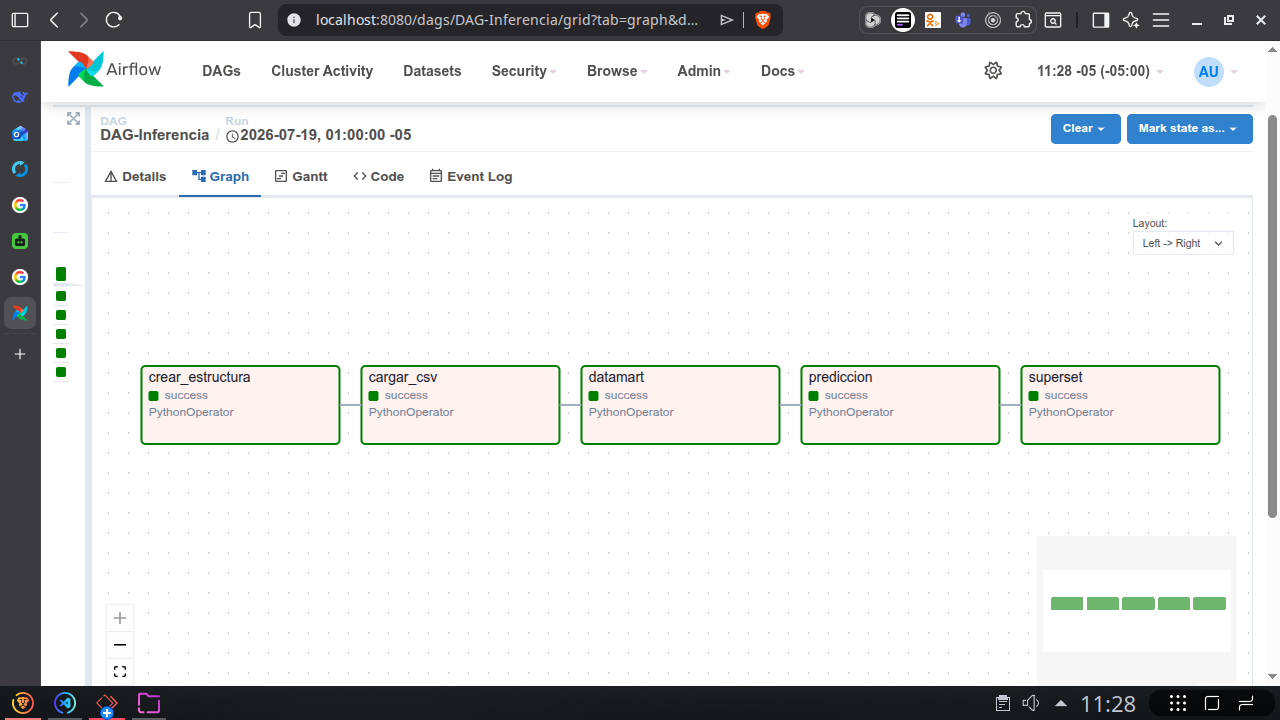
\includegraphics[width=0.8\textwidth]{images/dag-02inferencia.png}
    \caption{Vista del DAG de inferencia implementado en Apache Airflow.}
    \label{fig:dag_inferencia}
\end{figure}

\section{Datamart y dashboards}

La implementación almacena las predicciones en \texttt{fact\_predicciones\_mensual} y las expone mediante Apache Superset. Las Figuras 5.9--5.11 muestran ejemplos de los dashboards construidos.

\begin{figure}[H]
    \centering
    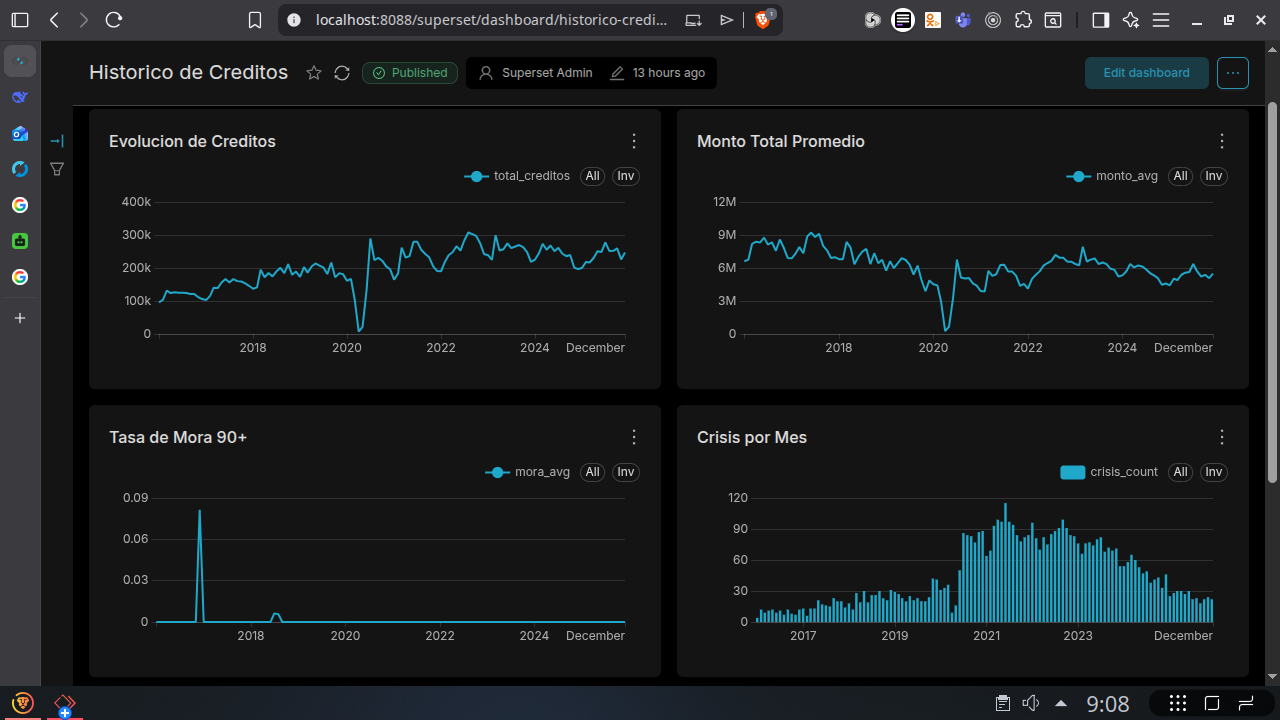
\includegraphics[width=0.8\textwidth]{images/dw-01-historicoCreditos1.png}
    \caption{Dashboard para el análisis histórico de la cartera crediticia.}
    \label{fig:dashboard_historico}
\end{figure}

Las capturas demuestran que las vistas fueron implementadas, pero no constituyen una validación de utilidad. No se reportan tiempos de actualización, pruebas de integridad, disponibilidad, errores, número de usuarios ni estudios de usabilidad. La afirmación defendible es que el prototipo integra visualmente datos históricos y predicciones; su impacto en decisiones y mora requiere evaluación posterior.

\section{Discusión}

Los resultados disponibles favorecen a LightGBM en el escenario evaluado, lo que es compatible con trabajos que reportan buen desempeño de modelos de boosting en datos tabulares \cite{lessmann2015benchmarking, moscato2021benchmark}. Sin embargo, la literatura también incluye escenarios en los que un MLP supera a los árboles \cite{gunnarsson2021deep}. Por ello, las diferencias observadas deben atribuirse al conjunto de datos y a las configuraciones utilizadas, no a una propiedad universal de los algoritmos.\\

El deterioro con el horizonte es visible en AUC-ROC y, con mayor intensidad, en recall. La cifra de recall igual a 0,034 a dieciocho meses significa que la clasificación binaria bajo el umbral 0,5 recupera una fracción muy pequeña de las crisis. Aunque el AUC-ROC se mantiene por encima de 0,70, no es suficiente para calificar estas predicciones como confiables o útiles sin análisis de umbral, calibración y costos de error.\\

El bajo rendimiento de CNN y MLP puede asociarse con la muestra secuencial reducida, el desbalance, las secuencias de seis meses y la configuración de entrenamiento. No obstante, no se realizaron ablaciones que modifiquen sistemáticamente estos factores. En consecuencia, se consideran explicaciones plausibles y no causas demostradas.\\

La principal fortaleza del trabajo es la integración de componentes. Su principal debilidad es la trazabilidad experimental. La ausencia de las reglas de etiqueta, de un diccionario completo, de un conjunto de validación documentado y de repeticiones limita la reproducibilidad y la generalización. Estas limitaciones deben resolverse antes de utilizar el sistema como soporte para decisiones de crédito en producción.